\subsection{IF Stage}

\begin{figure}[H]
\centering
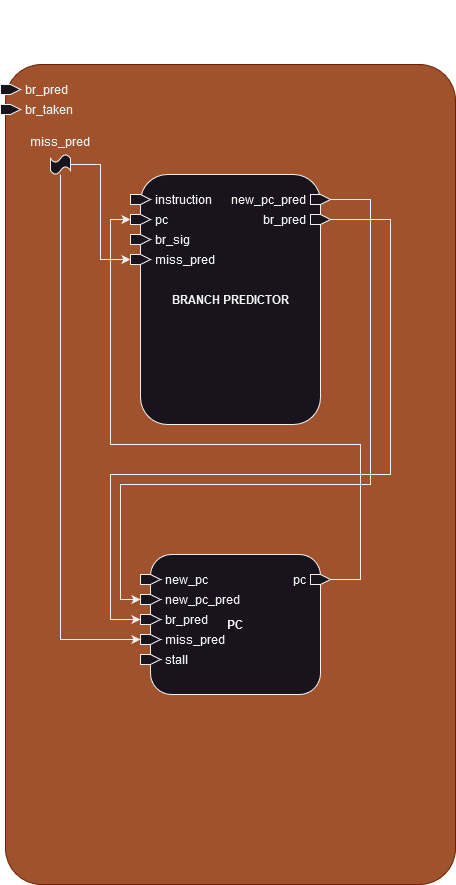
\includegraphics[width=0.5\textwidth]{../diagrams/fetch/if_stage.png}
\caption{Diagram of the IF Stage}
\label{fig:IF_Stage}
\end{figure}

The IF stage is responsible for fetching the next instruction from the ROM and passing it to the ID stage. 
The IF stage contains two different modules: the PC and the branch predictor.
The IF stage is the only stage that computes a value outside of a value, it uses the $br\_pred$ signal and the 
$br\_taken$ signal to compute if there is a miss prediction such that the PC and the branch predictor can be updated
accordingly. \\

Signals:
\begin{enumerate}
    \item Input: $br\_pred$, This signal is representing the state of the prediction made by the branch predictor in the EX stage.
    \item Input: $br\_taken$, This signal is representing the state of the branch in the EX stage.
    \item Output: $miss\_pred$, This signal is representing if there is a miss prediction or not.
\end{enumerate}
